\chapter[Evaluierung]{Evaluierung \small Daniel Mügge}\label{ch:eval}

Im Großen und Ganzen betrachtet ist \gamename ,umgangssprachlich ausgedrückt, ein rundes Ding.
Es gibt einige Dinge die sehr gut glaufen sind, einige Punkte auf die wir nicht unser Hauptaugenmerk gelegt haben und einige die wir einfach vergessen haben. Das kann vielleicht daran liegen das uns viele nützliche Features erst zu Ende des Projektes aufgefallen sind und uns schlicht und ergreifend die Zeit davon gelaufen ist. Zudem wurde JIRA eher schlecht als recht zum managen der Vorgänge und Sprints eingesetzt, wohingegen Git ein nützliches und kontinuierlich verwendetes Tool war.

Die Portierung des Spiels auf andere Plattformen außer Android, wie iOS und OS X, hat bis auf einige kleine Hürden problemlos funktioniert. Speziell für die plattformübergreifende Entwicklung ist cocos2d-x äußerst praktisch, weil die Engine den C$++$-Code selbstständig nativ übersetzt.
Das größte Problem war die unterschiedliche, erlaubte Pixelbreite von Bildern, was aber relativ schnell behoben war.

Auf die integrierte Physiks Engine von cocos2d-x haben wir verzichtet da unser Spiel nur von der Kollision zum Boden Gebrauch macht. Eine normale Physik Engine bezieht dafür noch viel mehr Parameter (bsp. Masse, Momentum, Gravitation) mit ein, was bei uns nicht gegeben ist oder mit einem unnötig hohen Mehraufwand verbunden.

Hinsichtlich der Performance haben wir uns auch wenig Gedanken gemacht. Hier bleibt noch offen Tests anzulegen um bestimmte Kriterien einzuhalten. Oder selbst einfache Tests zwischen zwei Funktionen durchzuführen. Beispielsweise ob es effektiver ist viele kleine Bilder nach Bedarf zu laden oder ein großes Bild ständig im Speicher zu halten. Des weiteren wäre zu klären ob die implementierte Kollisionsabfrage effektiv ist.

Die recht langen Ladezeit beim Starten eines Levels und besonders beim Starten des Zufallslevels sollte mit einem Lade-Bildschirm überdeckt werden, damit für den Endanwender ersichtlich ist, dass etwas im Gange ist.

Als Verbesserung des Ablaufs/Aufbaus der Animationen hätte man die Spawn Klasse von cocos2d verwenden können. Dadurch wäre eine variablere Verwendung von Sequenzen und Aktionen möglich. Diese hätte besonders bei den Angriffspattern der Boss Klasse Anwendung gefunden. Dadurch ist die komplette Boss Klasse momentan auf einen einzigen Endgegner fixiert.

Im Hinblick auf die Schwierigkeit und die Balance des Spiels war es für uns als Entwickler besonders schwer das Spiel neutral zu betrachten. Wenn dann haben wir es selbst getestet und nach einer gewissen Zeit weis man eben wie die Levels aussehen und wie die Steuerung einzusetzten ist. An dieser Stelle hätte man gezielte Langzeittests mit Unbeteiligten (sozusagen den Endanwendern) durchführen sollen. Wenn wir es Außenstehenden vorgestellt haben, dann nur kurz nebenbei um zu zeigen wie es aussieht.
Jedoch war bei den kurzen Tests schon zu sehen, dass unser Produkt ein relativ hohes, nennen wir es an dieser Stelle, "'Suchtpotential" hat. Alle Tester \textbf{wollten} die Levels schaffen und waren aufgrund von schwierigeren Passagen nicht gleich demotiviert.
\\Im Bezug auf den Schwierigkeitsgrad ist der Vorteil der "'festen"' Levels gegenüber dem zufällig generiertem Level, dass man diese einfach über den Editor, an Stellen die zu schwer sind, entschärfen kann. Jedoch muss man erwähnen das die Umsetzung des Zufallslevels sehr gut gelungen ist und außerdem wird man natürlich je nach Schwierikeitsgrad auch mit einer entsprechenden Anzahl an Münzen belohnt(1: 10, 2: 20, 3: 80).

\begin{figure}[H]
\centering
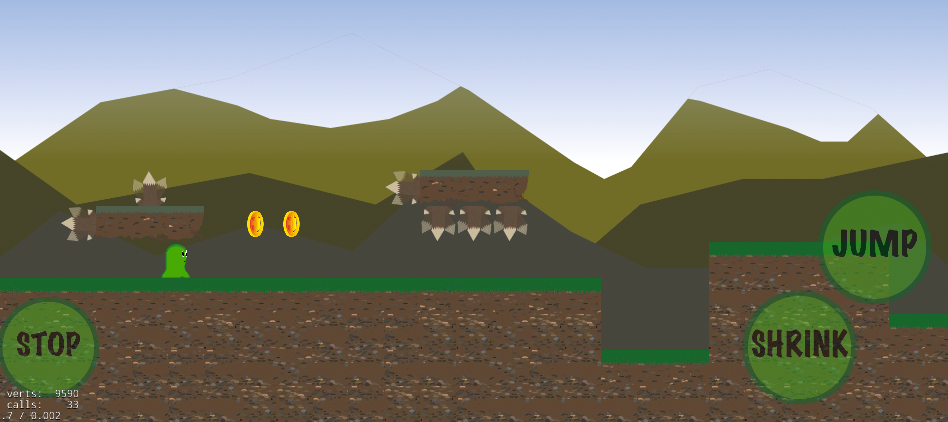
\includegraphics[width=12cm]{resources/randomdiff1}
\caption{Schwierige Passage bei Schwierigkeitsgrad 1}
\label{fig: randomdiff1}
\end{figure}


\begin{figure}[H]
\centering
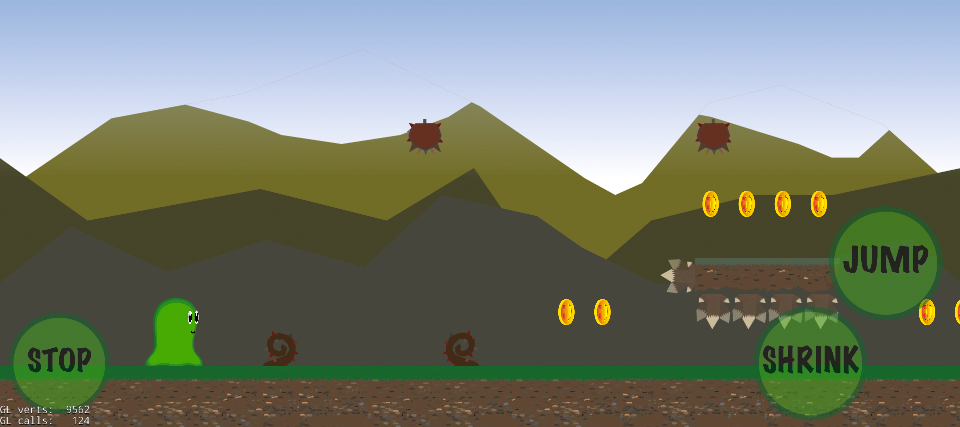
\includegraphics[width=12cm]{resources/randomdiff3}
\caption{Schwierige Passage bei Schwierigkeitsgrad 3}
\label{fig: randomdiff3}
\end{figure}

Die Implementierung des Sprungs bei \gamename ist für Erstanwender möglicherweise etwas gewöhnungsbedürftig, da es keine Mindestsprunghöhe gibt. Es wäre möglich diese zu implementieren jedoch haben wir während der Entwicklung festgestellt, dass das Spiel dadurch eine gewisse Individualität gegenüber anderen Spielen auf dem Markt erhält. Die restlichen Funktionalitäten der Steuerung weisen keine großen Besonderheiten auf und sind selbsterklärend, was sich weder positiv noch negativ auswirkt.

Ein Highlight des Spiels sind die Grafiken. Auch wenn es sich nicht hochkarätige 3D-Grafiken, sondern einfache 2D-Grafiken handelt, harmonieren sie mit dem Gesamtkonzept des Spiels. Sie wurden mit sehr viel Liebe zum Detail gestaltet und strahlen einen gewissen "'niedlichen"' charme aus. Diese Niedlichkeit ist genau das was wir bei \gamename haben wollten.
Ein gutes Beispiel dafür ist der Shop, in den man gelangt wenn man das Bosslevel startet. 

\begin{figure}[H]
\centering
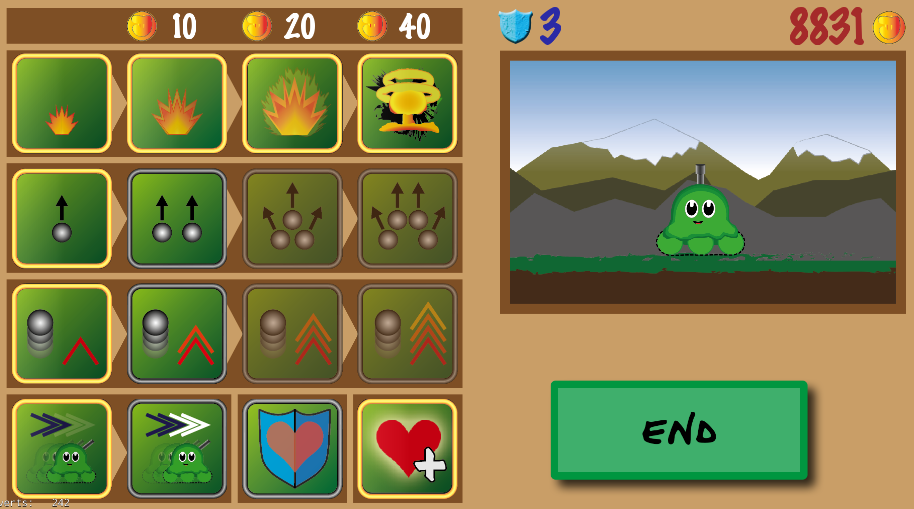
\includegraphics[width=16cm]{resources/shop}
\caption{Shop zum Erwerb von Aufwertungen für das Bosslevel}
\label{fig: shop}
\end{figure}